\section{Αριθμομηχανή}

Η ALU της προηγούμενης ενότητας χρησιμοποιείται για την δημιουργία της αριθμομηχανής του σχήματος \ref{schematic:calc}.
\begin{circuitfig}[H]
	\centering
	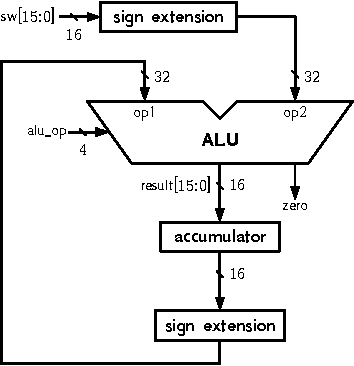
\includegraphics[width=6cm]{schematics/calc.pdf}
	\caption{Διάγραμμα ροής της αριθμομηχανής.}
	\label{schematic:calc}
\end{circuitfig}

\subsection{Module συσσωρευτή}
Τα 16 χαμηλότερα bit του αποτελέσματος της ALU περνάν ως είσοδος σε έναν συσσωρευτή των 16 bit. Ο συσσωρευτής λειτουργεί ως μνήμη της αριθμομηχανής και μηδενίζεται σύγχρονα με το πάτημα του άνω πλήκτρου και η τιμή του ενημερώνεται με κάθε πάτημα του κάτω πλήκτρου. Η έξοδός του συνδέεται με τα LED της αριθμομηχανής. Η υλοποίηση του συσσωρευτή περιγράφεται στο αρχείο \texttt{src/accum.v}. Το module \texttt{accum} έχει εισόδους το ρολόι, σήμα reset, σήμα για την ενημέρωση της τιμής του, τα δεδομένα προς αποθήκευση και ως έξοδο έχει τα δεδομένα τα οποία ήταν ήδη αποθηκευμένα.\par
Εντός ενός \texttt{always} block με τις ανερχόμενες ακμές του ρολογιού στη λίστα ευαισθησίας του, εκτελείται ένα block εμφολευμένων \texttt{if}. Ο πρώτος έλεγχος αφορά το reset, το οποίο αν είναι ενεργό η έξοδος του συσσωρευτή γίνεται μηδέν. Εάν το σήμα reset είναι ανενεργό ελέγχεται το σήμα update. Αν το update είναι ενεργό η τιμή της εξόδου λαμβάνει την τιμή της εισόδου, διαφορετικά η έξοδος διατηρεί την τιμή της.\par
% Η έξοδος του συσσωρευτή υφίσταται επέκταση προσήμου και θα είναι ο πρώτος τελεσταίος της ALU.\par

\subsection{Module αποκωδικοποιητή}
Η πράξη της ALU εισάγεται με συνδυασμό του αριστερού, δεξιού και κεντρικού πλήκτρου. Η αποδικοποίηση καθενός από τα τέσσερα bit του σήματος ελέγχου της ALU προκύπτει μέσω της λογικής των σχημάτων \ref{schematic:d0}, \ref{schematic:d1}, \ref{schematic:d2} και \ref{schematic:d3}.
\begin{circuitfig}[H]
	\centering
	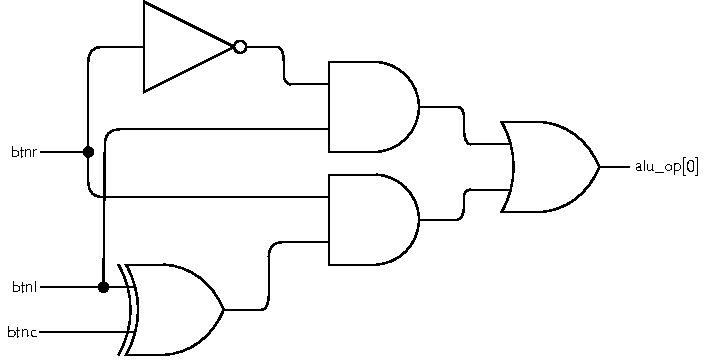
\includegraphics[width=8cm]{schematics/d0.pdf}
	\caption{LSB του σήματος ελέγχου της ALU.}
	\label{schematic:d0}
\end{circuitfig}
\begin{circuitfig}[H]
	% \vspace{0.5cm}
	\centering
	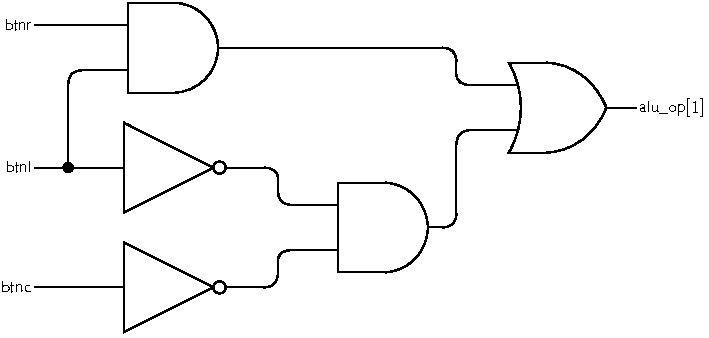
\includegraphics[width=8cm]{schematics/d1.pdf}
	\caption{Bit 2 του σήματος ελέγχου της ALU.}
	\label{schematic:d1}
\end{circuitfig}
\begin{circuitfig}[H]
	% \vspace{0.5cm}
	\centering
	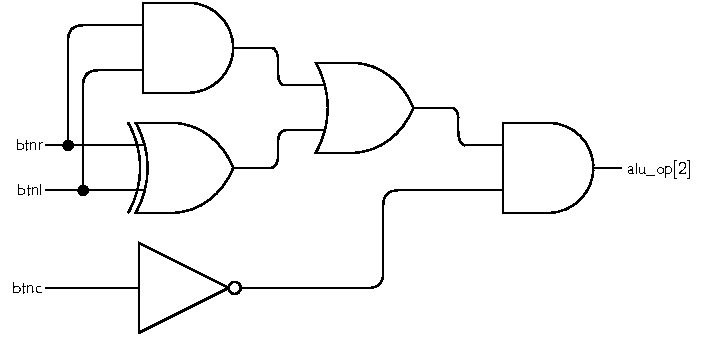
\includegraphics[width=8cm]{schematics/d2.pdf}
	\caption{Bit 3 του σήματος ελέγχου της ALU.}
	\label{schematic:d2}
\end{circuitfig}
\begin{circuitfig}[H]
	% \vspace{0.5cm}
	\centering
	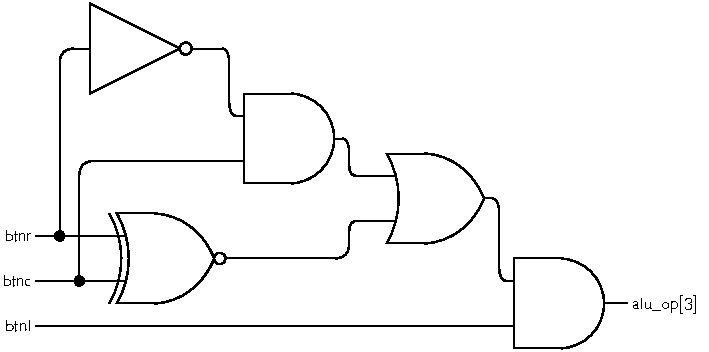
\includegraphics[width=8cm]{schematics/d3.pdf}
	\caption{MSB του σήματος ελέγχου της ALU.}
	\label{schematic:d3}
\end{circuitfig}

Οι μαθηματικές εκφράσεις που περιγράφουν τα παραπάνω σχήματα είναι
\begin{align}
	\text{alu\_op}[0] & =\(\lnot\text{btnr}\land\text{btnl}\)\lor\(\text{btnr}\land\(\text{btnl}\oplus\text{btnc}\)\)      \\
	\text{alu\_op}[1] & =\(\text{btnr}\land\text{btnl}\)\lor\(\lnot\text{btnl}\land\lnot\text{btnc}\)                      \\
	\text{alu\_op}[2] & =\(\(\text{btnr}\land\text{btnl}\)\lor\(\text{btnr}\oplus\text{btnl}\)\)\land\lnot\text{btnc}      \\
	\text{alu\_op}[3] & =\(\(\lnot\text{btnr}\land\text{btnc}\)\lor\lnot\(\text{btnr}\oplus\text{btnc}\)\)\land\text{btnl}
\end{align}

Στο αρχείο \texttt{src/decoder.v} ορίζεται ένα νέο module με όνομα \texttt{decoder} και εισόδους το κεντρικό, το αριστερό και το δεξί πλήκτρο. Η έξοδός του είναι τεσσάρων bit και αντιπροσωπεύει τον κωδικό της προς εκτέλεση πράξης της ALU.\par
Εντός ενός \texttt{always} block εφαρμόζονται οι παραπάνω σχέσεις χρήσει λογικών τελεστών της Verilog. Η λειτουργία, δηλαδή, του module περιγράφεται χρήσει structural Verilog.\par

\subsection{Module αριθμομηχανής}
Στο αρχείο \texttt{src/calc.v} ορίζεται ένα module με όνομα \texttt{calc} με εισόδους το ρολόι, πέντε πλήκτρα (κεντρικό, δεξί, αριστερό, άνω, κάτω), δεδομένα των 16 bit (δεύτερος τελεσταίος) και έξοδο σε LED.\par
Γίνεται instantiate του συσσωρευτή, της ALU και του αποκωδικοποιητή. Ως σήμα reset στον συσσωρευτή εφαρμόζεται το άνω πλήκτρο και ως update το κάτω πλήκτρο. Στην ALU, ως σήμα ελέγχου εφαρμόζεται η έξοδος του αποκωδικοποιητή.\par
Εντός ενός \texttt{always} block, τα 16 χαμηλότερα bit του αποτελέσματος της ALU συνδέονται στην είσοδο του συσσωρευτή. Η έξοδος του συσσωρευτή συνδέεται στα LED της αριθμομηχανής. Επιπλέον, γίνεται επέκταση προσήμου της τιμής των LED και το αποτέλεσμα συνδέεται στον πρώτο τελεσταίο της ALU. Ο δεύτερος τελεσταίος της ALU συνδέεται με τους διακόπτες δεδομένων μετά από επέκταση προσήμου.\par

\subsection{Testbench}

Στο αρχείο \texttt{src/calc\_TB.v}, αρχικά γίνεται instantiate η αριθμομηχανή. Έπειτα, σε ένα \texttt{initial} block μηδενίζεται το ρολόι, ενεργοποιείται το άνω πλήκτρο (reset) και στους διακόπτες δεδομένων δίνεται η αρχική τιμή $\(1234\)_{\mathrm{HEX}}$. Μετά από $20\unit{\nano\second}$ το reset απενεργοποιείται.\par
Σε ένα \texttt{always} block χωρίς λίστα ευαισθησίας ανά $10\unit{\nano\second}$ η τιμή του ρολογιού συμπληρώνεται. Συνεπώς, η περίοδος είναι $T=20\unit{\nano\second}$.\par
Σε ένα δεύτερο \texttt{always} block χωρίς λίστα ευαισθησίας ρυθμίζεται το κάτω πλήκτρο (update) ώστε να ενεργοποιείται $1\unit{\nano\second}$ πριν τη θετική ακμή του ρολογιού και να απενεργοποιείται $2\unit{\nano\second}$ μετά.\par
Εντός ενός δεύτερου \texttt{initial} block, μετά από $29\unit{\nano\second}$ ($1\unit{\nano\second}$ πριν τη θετική ακμή του ρολογιού) ρυθμίζονται το αριστερό, κεντρικό και δεξί πλήκτρο για την πράξη της λογικής διάζευξης. Έπειτα, ανά $20\unit{\nano\second}$ ρυθμίζονται εκ νέου τα πλήκτρα και οι διακόπτες δεδομένων. Το χρονοδιάγραμμα φαίνεται στο διάγραμμα \ref{diagram:calc}.\par

\begin{plotenv}[H]
	\centering
	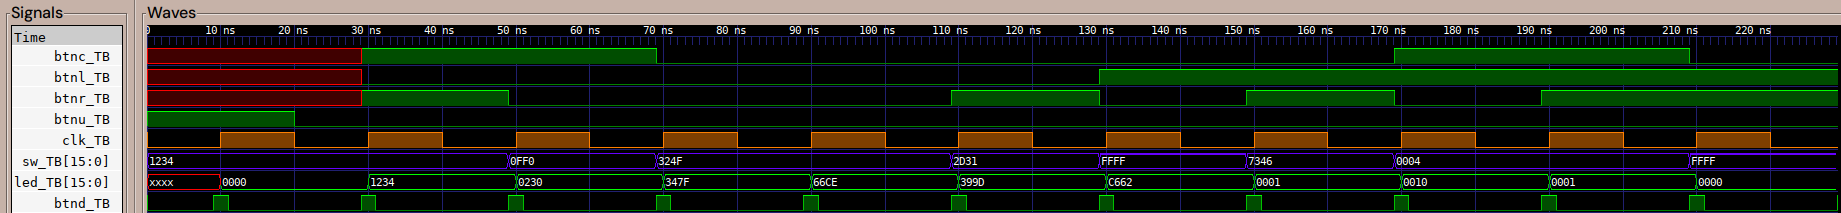
\includegraphics[width=\linewidth]{waveforms/calc.png}
	\caption{Χρονοδιάγραμμα για το testbench της αριθμομηχανής. Επιβεβαιώνεται η ορθή λειτουργία της αριθμομηχανής.}
	\label{diagram:calc}
\end{plotenv}